\begin{figure}[t]
\centering
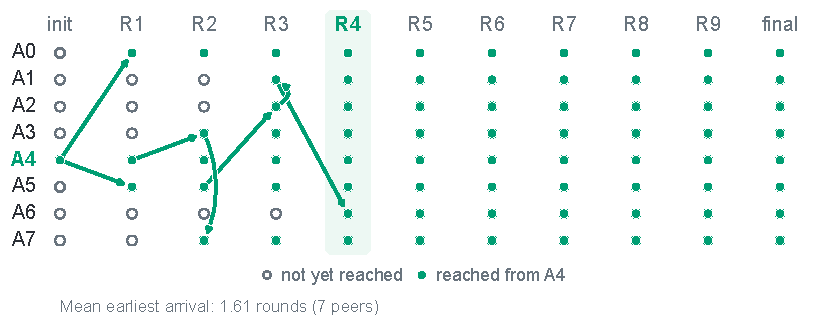
\includegraphics[width=\linewidth]{../paper/figures/final/fig6.pdf}
\caption{\textbf{Potential information spread from A4.}
For the selected $N=8$ schedule, green nodes indicate agents reachable from A4
by a time-respecting path; arrows show the seven first-arrival contacts.
Same-round relays retain the original message ordering. The mean earliest
arrival over the seven peers, excluding A4, is $90/(7\times8)\simeq1.61$
rounds. All peers are reached after message 26 (3.25 rounds), hence by R4.
The final column is R10. Reach describes potential information transmission,
not measured belief adoption.}
\label{fig:social-circuit}
\end{figure}
